
  \section{Zielsetzung}

    In diesem Versuch soll die Lebensdauer von kosmischen Myonen,
    welche in einem Szintillator abgebremst werden und dort zerfallen,
    bestimmt werden. Dies wird realisiert, indem viele individuelle Lebensdauern
    mithilfe einer elektrischen Schaltung
    aufgezeichnet werden und daraus eine allgemeine Lebensdauer bestimmt wird.


  \section{Theorie}

    \subsection{Myonen}

    Myonen sind Elementarteilchen und gehören zur Familie der Leptonen.
    Auf sie wirken die schwache und die elektromagnetische Wechselwirkung.
    Ihre Masse beträgt in etwa das 200-fache der Elektronenmasse.
    Wenn Pionen, die erzeugt werden, wenn energiereiche kosmische Protonen
    mit Luftmolekülen in Wechselwirkung treten, zerfallen, entstehen Myonen.
    Beim Zerfall von einem $\pi^-$ entsteht ein Myon und beim Zerfall von
    einem $\pi^+$ ein Antimyon. Die Zerfallsgleichungen lauten
    \begin{align*}
      &\pi^+ \to \mu^+ +\nu_{\mu}\\
      &\pi^- \to \mu^- +\bar{\nu}_{\mu}\,\,\,\,.
    \end{align*}
    Von diesen Myonen gelangen einige, die nahezu Lichtgeschwindigkeit
    besitzen, zur Erde. Ihre kinetische Energie kann bei mehreren Hundert MeV
    liegen. \\
    Myonen zerfallen in Elektronen bzw. Positronen und Neutrinos gemäß den Gleichungen
    \begin{align*}
      &\mu^- \to e^- +\bar{\nu}_e+\nu_{\mu}\\
      &\mu^+ \to e^+ +\nu_e +\bar{\nu}_{\mu}\,\,\,\,.
    \end{align*}
    Die Lebensdauer von Myonen beträgt in etwa $2,2\,\mu$s~\cite{pdg}.

    \subsection{Lebensdauer eines instabilen Teilchens}

    Wenn die Lebensdauer eines einzelnen Teilchens gemessen wird,
    kann aus dem Ergebnis kein Rückschluss auf die Lebensdauer
    anderer Teilchen gezogen werden, weil die individuellen Lebensdauern
    statistisch verteilt sind. \\
    Die Lebensdauer $\tau$ einer Teilchenart beschreibt die Zeit, nach welcher
    die ursprüngliche Teilchenmenge $N_0$ auf den Wert $\frac{N_0}e$ reduziert
    wurde. Ihr Kehrwert ist die Zerfallskonstante $\lambda.$\\
    Die Wahrscheinlichkeit für den Zerfall eines Teilchens im Intervall $dt$ ist
    $dW=\lambda\,dt.$\\
    Wird die Teilchenzahl mit einbezogen, entsteht die Gleichung
    \begin{align*}
      \frac{dN}{dt}=-\lambda N.
    \end{align*}
    Daraus lässt sich eine genäherte Formel für die zeitliche Entwicklung der
    Teilchenzahl herleiten:
    \begin{align*}
      N(t)=N_0\symup{e}^{-\lambda t}=N_0\symup{e}^{-t/\tau}.
    \end{align*}
    Um aus einer Stichprobe von $n$ Lebensdauern $\tau$ zu bestimmen,
    ist es sinnvoll, die Methode der kleinsten Quadrate anzuwenden.
    Dabei wird der Ausdruck
    \begin{align*}
      \sum_{j=1}^n \left(N(t_j)-N_0\,\symup{e}^{-\lambda t}\right)²
    \end{align*}
    minimalisiert, indem $N_0$ und $\lambda$ verändert werden.
    Die Zeit $t_j$ wurde in der Stichprobe $N(t_j)$ mal gemessen.



  \section{Aufbau}

    \begin{figure}[H]
      \centering
      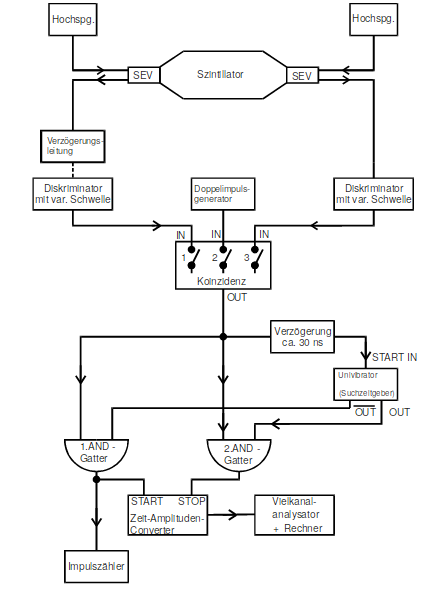
\includegraphics[height=10cm]{myonaufbau.png}
      \caption{Schaltung zur Lebensdauermessung kosmischer Myonen~\cite{anleitung}.}
      \label{fig:schaltung}
    \end{figure}


    In Abbildung \ref{fig:schaltung} ist eine Schaltung zu sehen,
    mit welcher die Lebensdauer kosmischer Myonen bestimmt werden kann.
    Dabei ist zu berücksichtigen, dass auf der rechten Seite
    zwischen SEV und Diskriminator ebenfalls eine Verzögerung eingebaut ist.\\
    \ \\
    Ein wesentlicher Baustein der Schaltung ist der \textbf{Szintillationsdetektor}.
    Dies ist ein 50\,l umfassender Edelstahltank gefüllt mit Tuolol,
    in dem Lichtimpulse nach etwa 10\,ns abklingen.
    Ein eintreffendes Myon regt durch seine hohe kinetische Energie von
    teilweise mehr als 100\,MeV die Moleküle im Szintillator an, welche
    beim Zurückfallen in den Ursprungszustand Lichtquanten emittieren.
    Wenn ein Myon im Szintillator zerfällt, entsteht ein Elektron oder ein
    Positron, welches ebenfalls genug Energie besitzt, um die Szintillatormoleküle
    entsprechend anzuregen. \\
    Die \textbf{Sekundärelektronenvervielfacher} (kurz SEV) mit eingebauten
    \textbf{Photokathoden} an beiden Enden des Szintillators bewirken,
    dass die eintreffenden Lichtimpulse in elektrische Signale umgewandelt
    werden.\\
    Um die leicht unterschiedlichen Eigenschaften der beiden SEV ausgleichen
    zu können, wird nach jedem SEV eine \textbf{Verzögerungsleitung} eingebaut.
    Im Prinzip besteht die Leitung aus vielen einzelnen Kabeln, die einzeln dazugeschaltet
    werden können, um die Stromstrecke zu verlängern. \\
    Nach jeder Verzögerungsleitung folgt ein \textbf{Diskriminator}. An diesem können zwei
    Dinge eingestellt werden. Zunächst einmal ist die Mindestspannungshöhe
    einstellbar, die ein Impuls haben muss, um vom Diskriminator
    durchgelassen zu werden. Dies sorgt für eine erste Herausfilterung
    ungewünschter Spannungsimpulse, welche durch eine spontane Elektronenemission
    von einer der Photokathoden entstehen können, da einigie von ihnen viel kleiner
    sind als die Myonenimpulse. Außerdem kann am Diskriminator
    eingestellt werden, wie lang der Rechteckimpuls sein
    soll, welcher aus dem SEV-Impuls entsteht.\\
    Die nachfolgende \textbf{Koinzidenzschaltung} dient dazu, einen noch größeren Teil
    der unerwünschten Elektronenimpulse herauszufiltern. Die zugrundeliegende
    Annahme ist, dass ein durch spontane Elektronenemission erzeugter Impuls
    nur an einem SEV einen Spannungsimpuls auslöst, ein durch ein Myon erzeugter
    Lichtblitz aber in einer sehr kleinen Zeit bei beiden SEV zu einer Reaktion
    führt. Die Koinzidenzschaltung lässt folglich nur
    "gleichzeitige" Ereignisse passieren.
    Findet ein Lichtblitz ganz nah bei einem der SEV statt, wird an
    diesem SEV quasi sofort ein Spannungssignal erzeugt. Es wird
    vom Diskriminator in ein Rechtecksignal umgewandelt.
    Am anderen SEV kommt das Licht etwas später an.
    Der dort erzeugte Spannungsimpuls des SEV wird vom nachgeschalteten
    Diskriminator ebenfalls in ein Rechtecksignal umgewandelt.
    Die Koinzidenzschaltung erkennt die Ereignisse
    als gleichzeitig an, die zu sich überlappenden Rechtecksspannungssignalen
    der beiden SEV führen.\\
    Nachdem nun annähernd gewährleistet ist, dass nach der Koinzidenzschaltung
    nur noch verwertbare Signale vorliegen, muss ein Mechanismus eingesetzt
    werden, der dazu führt, dass das Signal des eintreffenden Myons die
    Lebensdauermessung startet, und dass der Zerfall die Messung beendet. \\
    Dazu wird das aus der Koinzidenzschaltung kommende Signal an einen Eingang
    des 1.AND-Gatters und an einen Eingang des 2.AND-Gatters weitergeleitet.
    Der zweite Ausgang der \textbf{AND-Gatter} ist mit einer
    \textbf{monostabilen
    Kippstufe} verbunden.
    AND-Gatter lassen ein Signal nur passieren, wenn auf ihre beiden
    Eingänge das Signal HIGH gegeben wird. Wenn an einem Eingang ein
    Spannungsimpuls ankommt, liegt an diesem Eingang für die Dauer
    des Impulses ein HIGH an.\\
    In die Kippstufe fließt ebenfalls das Signal aus der Koinzidenzschaltung, allerdings
    ist eine Verzögerung eingebaut, sodass das Signal im Vergleich zu den AND-Gattern
    erst etwa 30\,ns später ankommt.\\
    Im Grundzustand ist die Kippstufe so eingestellt, dass sie auf den Eingang
    des 1.AND-Gatters ein HIGH gibt, auf den des 2. ein LOW.
    Kommt jetzt ein Startimpuls durch ein Myon hinter der Koinzidenzschaltung
    an, fließt er in beide AND-Gatter und sorgt für ein HIGH auf dem ersten
    Eingang. Beim 1.AND-Gatter liegt durch die Kippstufe auf dem zweiten
    Eingang ebenfalls ein HIGH, sodass der Impuls hindurchgeht und
    als Startimpuls gezählt wird.
    Beim 2.AND-Gatter liegt durch die Kippstufe am zweiten Eingang ein LOW an,
    weshalb das Signal nicht passieren kann.\\
    Nach 30\,ns, wenn der Impuls an den ersten Eingängen der AND-Gatter
    schon wieder weg ist, erreicht das Signal aus der Koinzidenzschaltung
    die monostabile Kippstufe und führt dazu, dass diese sich umkehrt.
    Sie gibt nun also ein LOW auf den zweiten Eingang des 1.AND-Gatters und ein
    HIGH auf den zweiten Eingang des 2.AND-Gatters. \\
    Kommt jetzt durch die Koinzidenzschaltung ein Signal durch den Myonenzerfall,
    wird es wieder zu den beiden AND-Gattern geleitet. Allerdings kann es
    diesmal aufgrund der Änderung der Situation durch die Kippstufe
    nur das 2.AND-Gatter passieren und wird somit als Stop-Impuls gezählt.\\
    Der Stop-Impuls nach 30\,ns Verzögerung führt dazu, dass
    die Kippstufe wieder zurückkippt, sodass ein neuer Startimpuls auch
    als solcher erkannt wird.\\
    Start- und Stop-Impulse werden beide vom \textbf{Zeit-Amplituden-Converter}
    (kurz TAC) registriert. Dieser berechnet dann die Zeit zwischen Start-
    und Stop-Impuls und wandelt die Länge der Zeit in ein dazu proportionales
    Spannungssignal um. \\
    Diese Spannungssignale werden ihrer Höhe entsprechend in einem Kanal
    des \textbf{Vielkanalanalysators} gespeichert.\\
    Ein angschlossener Rechner implementiert die in der Theorie
    vorgestellte Methode zur Berechnung der Lebensdauer.\\
    Da einige Myonen eine hohe Geschwindigkeit haben, und somit den
    Szintillator wieder verlassen, ohne in ihm zu zerfallen, muss verhindert
    werden, dass ein zweites einfallendes Myon als Stop-Impuls für
    ein durchgeflogenes Myon gewertet wird. Dazu wird die Suchzeit $T_S$
    eingeführt. In dieser Zeit läuft die Schaltung wie zuvor beschrieben. Trifft
    allerdings in der Suchzeit kein Stop-Impuls ein, wird die Apparatur
    zurückgesetzt und wartet auf einen neuen Startimpuls.
    Die Suchzeit sollte so gewählt werden, dass es unwahrscheinlich ist,
    dass in ihr 2 Myonen im Tank eintreffen.\\
    Um die Startimpulse ohne zugehörige Stop-Impulse trotzdem registrieren zu
    können, wird zwischen dem 1.AND-Gatter und dem Eingang des
    TAC ein Impulszähler eingebaut.\\
    Damit die vom TAC berechneten Werte überprüft werden können,
    kann zwischen dem 2.AND-Gatter und dem TAC ebenfalls ein Impulszähler
    eingebaut werden.\\
    Der Doppelimpulsgenerator, welcher ebenfalls an die Koinzidenzschaltung
    angeschlossen ist, hat für die eigentliche Registrierung von Myonen
    keine Bewandnis. Er dient lediglich zur Kalibrierung.

  \section{Durchführung}

    Zunächst wird Hochspannung auf den Szintillator gegeben. Mithilfe eines
    Oszilloskops, an dessen Eingängen ein \SI{50}{\ohm}-Widerstand zur
    Reflexionsvermeidung eingebaut ist, kann überprüft werden, ob die
    SEV Spannungsimpulse aussenden.\\
    Nun werden die Diskriminatoren angeschlossen. Das Oszilloskop
    sollte Rechtecksignale anzeigen.\\
    Zur Einstellung der Diskriminatorschwelle wird der
    Impulszähler, der einfallende Myonen zählt, angeschlossen.
    Die Widerstände der Diskriminatoren werden so lange verändert, bis in einer
    10-sekündigen Messung etwa 350 Myoneneinfälle pro SEV detektiert werden,
    was 35 Myoneneinfällen pro Sekunde entspricht.\\
    Jetzt wird mithilfe der Diskriminatoren eingestellt,
    wie lang das Rechtecksignal sein soll, welches aus einem SEV-Signal
    im Diskriminator erzeugt wird. Die Länge des Plateaus wird bei
    beiden SEV auf etwa 12\,ns eingestellt.\\
    Danach werden die aus den Diskriminatoren kommenden Kabel
    in die Koinzidenzschaltung gesteckt.\\
    Um die Ungleichheiten der beiden SEV auszugleichen, wird hinter
    jedes SEV eine Verzögerungsleitung eingebaut. Eine der Verzögerungsleitungen
    wird zunächst nicht benutzt, während die Länge der anderen so
    variiert wird,
    dass die durch sie verursachte Verzögerung im Bereich von 1 bis 30\,ns
    liegt. In 1\,ns-Schritten wird die Verzögerung erhöht und zu jeder
    Verzögerungszeit die Anzahl der einfallenden Myonen pro 10\,s gemessen.
    Im Anschluss wird die gleiche Messung noch einmal vorgenommen,
    mit dem Unterschied, dass diesmal die Länge der ersten Verzögerungsleitung
    variiert wird und die für das zweite SEV nicht verwendet wird.
    Es wird überprüft, für welchen eingestellten Widerstand die nach der
    Koinzidenzschaltung gemessene Anzahl der einfallenden Myonen am größten ist.
    Da die Diskriminatoren Rechteckimpulse aussenden, gibt es theoretisch nicht
    einen Maximalwert, sondern ein Plateau von Maximalwerten. In der
    Praxis liegt der Maximalwert der verwendeten Apparatur bei 276 einfallenden
    Myonen pro 10\,s und kommt genau dann vor, wenn nach dem 2.SEV eine Verzögerung
    von 8\,ns eingestellt ist. Der Maximalwert bestätigt ebenfalls die Funktion
    der Koinzidenzschaltung, da sich die Zahl der pro Sekunde ankommenden
    Myonen von etwa 35 (ohne Koinzidenz) auf etwa 28 reduziert hat.\\
    Ein Ausgang der Koinzidenzschaltung wird, mit einem zwischengeschalteten
    Widerstand, der eine Verzögerung von 30\,ns bewirkt, an die monostabile
    Kippstufe angeschlossen. Die Suchzeit wird an der Kippstufe auf 13\,$\mu$s
    eingestellt.\\
    Danach werden die anderen Ausgänge der Koinzidenzschaltung
    mit den ersten Eingängen der AND-Gatter verbunden.
    Der $\overline{\symup{OUT}}$-Ausgang der Kippstufe wird auf den zweiten
    Eingang des 1.AND-Gatters gegeben, der OUT-Ausgang wird auf den zweiten
    Eingang des 2.AND-Gatters gegeben.\\
    Beide Ausgänge der AND-Gatter führen (über jeweils einen Impulszähler)
    in den TAC, wobei das 1.AND-Gatter auf den Start- und das 2.AND-Gatter
    auf den Stop-Eingang gegeben wird. \\
    An den TAC werden ein Vielkanalanalysator und ein Rechner angeschlossen.\\
    Die Fuktion des TAC wird überprüft, indem anstelle der beiden SEV
    der Doppelimpulsgenerator auf einen Eingang der Koinzidenzschaltung gegeben wird.
    Dieser generiert Doppelimpulse, deren Zeitabstand in einem Bereich
    von 0,1 bis 9,9\,$\mu$s manuell eingestellt werden kann.
    Um eine Aussage darüber treffen zu können, welcher Kanal für welchen
    Zeitabstand zwischen den Impulsen steht, wird die Frequenz des
    Doppelimpulsgenerators immer in 0,5\,$\mu$s-Schritten erhöht, und beobachtet,
    welcher Zeitabstand der Impulse welchen Kanal füllt.
